\section{Sampling and Reconstruction\buch{Chapter 1}}
\subsection{Analog Signals\buchSeite{2}}
\begin{tabular}{llp{3cm}ll}
  $\Omega = 2\pi f$ & $[\Omega] = \frac{rad}{s}$ & &
  $\omega = \Omega T = \frac{2\pi f}{f_s}$ & $[\omega] = \frac{rad}{sample}$
\end{tabular}

\begin{tabularx}{\linewidth}{|l|X|}
	\hline
	Fourier transform & $X(\Omega) = \int\limits_{-\infty}^{\infty} x(t)e^{-j\Omega t}dt$ \\
	\hline
	inverse Fourier transform & $ x(t) = \int\limits_{-\infty}^{\infty} X(\Omega)e^{j\Omega t} \frac{d\Omega}{2 \pi} $ \\
	\hline
\end{tabularx}

\subsection{Digital Signals}
\subsubsection{Sampling Theorem\buchSeite{4-6}}
Sampling means that the analog signal is periodically measured with a sampling interval T. The discrete index $n$, relates to
the time $t$ as follows:
\[ t = nT \qquad n = 0,1,2,\ldots \]
The sampling frequency relates to the sampling interval as follows:
\[ f_s = \frac{1}{T} \]
\begin{multicols}{2}
  Sampling Theorem (Nyquist rate):
  \[ f_s \geq 2f_{max} \qquad \text{or} \qquad T \leq \frac{1}{2f_{max}} \]
  
\columnbreak

  Nyquist interval:
  \[ \left[-\frac{f_s}{2}, \frac{f_s}{2}\right] \]
  
\end{multicols}

%The spectrum $\hat{X}(f)$ of the sampled signal will be replicated
%\[ \hat{X}(f) = \frac{1}{T} \sum_{m=-\infty}^{\infty}X(f-m f_s)\]


\subsubsection{DSP Frequency Units\buchSeite{29-30}}
A sampled sinusoid takes the form in these units:
\[
	e^{2\pi jfTn} = e^{2\pi j (f/f_s)n} = e^{j\Omega Tn} = e^{j\omega n}
\]

\begin{center}
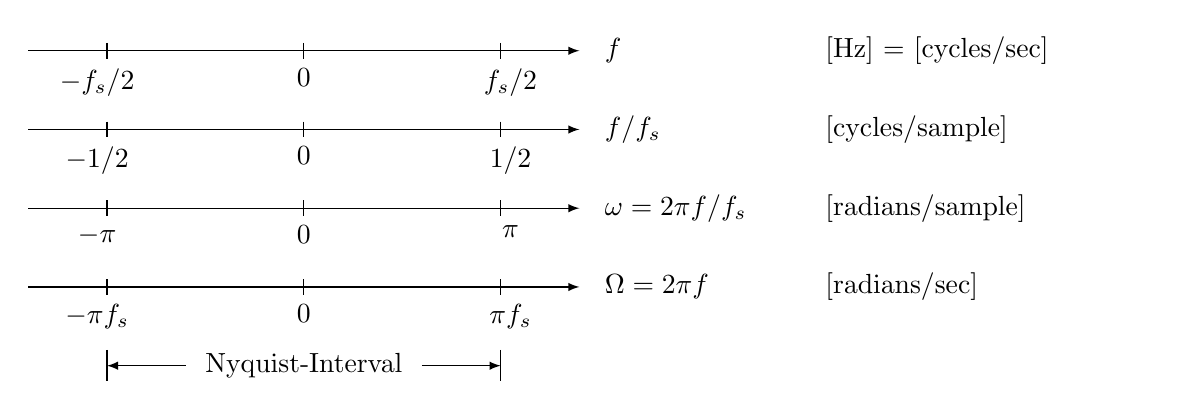
\begin{tikzpicture}
	\draw[-latex] (0,0) -- ++(7,0)
		node[midway, below={0.1cm}] {0}
		node[very near start, below={0.1cm}] {$-\pi f_s$}
		node[very near end, below={0.1cm}] {$\pi f_s$}
		node[at end, right={0.2cm}] {$\Omega = 2 \pi f$}
		node[at end, right={3cm}, text width=4cm] {[radians/sec]};
	\draw[-latex] (0,1) -- ++(7,0)
		node[midway, below={0.1cm}] {0}
		node[very near start, below={0.1cm}] {$-\pi$}
		node[very near end, below={0.1cm}] {$\pi$}
		node[at end, right={0.2cm}] {$\omega = 2 \pi f/f_s$}
	    node[at end, right={3cm}, text width=4cm] {[radians/sample]};
	\draw[-latex] (0,2) -- ++(7,0)
		node[midway, below={0.1cm}] {0}
		node[very near start, below={0.1cm}] {$-1/2$}
		node[very near end, below={0.1cm}] {$1/2$}
		node[at end, right={0.2cm}] {$f/f_s$}
		node[at end, right={3cm}, text width=4cm] {[cycles/sample]};
	\draw[-latex] (0,3) -- ++(7,0)
		node[midway, below={0.1cm}] {0}
		node[very near start, below={0.1cm}] {$-f_s/2$}
		node[very near end, below={0.1cm}] {$f_s/2$}
		node[at end, right={0.2cm}] {$f$}
		node[at end, right={3cm}, text width=4cm] {[Hz] = [cycles/sec]};
	% Markierungen
	\draw (1,0.1) -- +(0,-0.2)
		(3.5,0.1) -- +(0,-0.2)
		(6,0.1) -- +(0,-0.2);
	\draw (1,1.1) -- +(0,-0.2)
		(3.5,1.1) -- +(0,-0.2)
		(6,1.1) -- +(0,-0.2);
	\draw (1,2.1) -- +(0,-0.2)
		(3.5,2.1) -- +(0,-0.2)
		(6,2.1) -- +(0,-0.2);
	\draw (1,3.1) -- +(0,-0.2)
		(3.5,3.1) -- +(0,-0.2)
		(6,3.1) -- +(0,-0.2);
	% Anmerkung Nyquist Interval
	\draw (1,-0.8) -- +(0,-0.4)
		(6,-0.8) -- +(0,-0.4);
	\draw[-latex] (2,-1) -- +(-1,0);
	\draw[-latex] (5,-1) -- +(1,0);
	\node at(3.5, -1) {Nyquist-Interval};
\end{tikzpicture}
\end{center}

\subsubsection{Flat-top sampling \buchSeite{30}}
In practical sampling each sample is held for a short period of time ($\tau$).
\[ x_{flat}(t) =  \sum_{n=-\infty}^{\infty}x(nT)p(t - nT) \qquad p(t) \text{: flat-top pulse with duration } \tau \]

This is equivalent to filtering the perfectly sampled signal $\hat{x}$ with a linear filter with the impulse response $p(t)$.
The spectrum of the filter looks like this
\[ |P(f)| = \tau \left| \frac{sin(\pi f \tau)}{\pi f \tau} \right| \]
% TODO maybe add plot

\subsubsection{Discrete-Time Fourier Transform (DTFT)\buchSeite{31}}
\[
	\hat{X}(f) = \sum_{n=-\infty}^{\infty} x(nT)e^{-2\pi jfTn}
\]
\[
	x(nT) = \frac{1}{f_s} \int_{-f_s/2}^{f_s/2}\hat{X}(f)e^{2\pi jfTn}df = \int_{-\pi}^{\pi}\hat{X}(\omega)e^{j\omega n} \frac{d \omega}{2 \pi}
\]

  A sampled signal has always a periodic spectrum, with its spectrum center at the multiplies of the sampling frequency.\\
  $\hat{X}(f) = \frac{1}{T}\sum\limits_{m=-\infty}^{\infty}X(f-mf_s) \qquad \qquad
  T\hat{X}(f) = X(f) \quad$ for $-\frac{f_s}{2} \leq f \leq \frac{f_s}{2}$





\subsubsection{Aliasing\buchSeite{10, 38}}
If the signal frequency $f$ is outside the Nyquist interval, the signal will be
aliased with $f - f_{sampling}$.\\

\textbf{Example:} $sin(8\pi t)$ (signal frequency $f=4$) sampled at a rate of
$f_s=5Hz$ will be aliased to $sin(2\pi (f-f_s) t) = sin(2\pi (-1) t)$
\[ f_{ia} = f_i + nf_s \]
n has to be choosed, that $f_{ia}$ is in the Nyquist intervall. n can also be negative.\\


Is the signal frequency $f$ inside the Nyquist interval $\left[-f_s/2,+f_s/2\right]$, no aliasing will be
perceived.

\subsubsection{Antialiasing Prefilter \buchSeite{38}}
The stop frequency from the antialiasing prefilter is defined as:
\[ f_{stop} = f_s - f_{pass} \]
The attenuation of the antialiasing prefilter is:
\begin{multicols}{2}

\[ A(f) = -20 \cdot \log_{10}{\left|\frac{H(f)}{H(f_0)}\right|} \qquad [dB] \]

\[ A_{dB} = \alpha \log_{10}(\frac{f}{f_{cutoff}}) \qquad \alpha = \frac{dB}{dek} \]

\[ A_{dB} = \beta \log_{2}(\frac{f}{f_{cutoff}}) \qquad \beta = \frac{dB}{okt} \]

\[ A_{X}(f) = \underbrace{A(f)}_{Prefilter} + \underbrace{A_{X_{in}}(f)}_{Input spectrum} \]

\columnbreak

 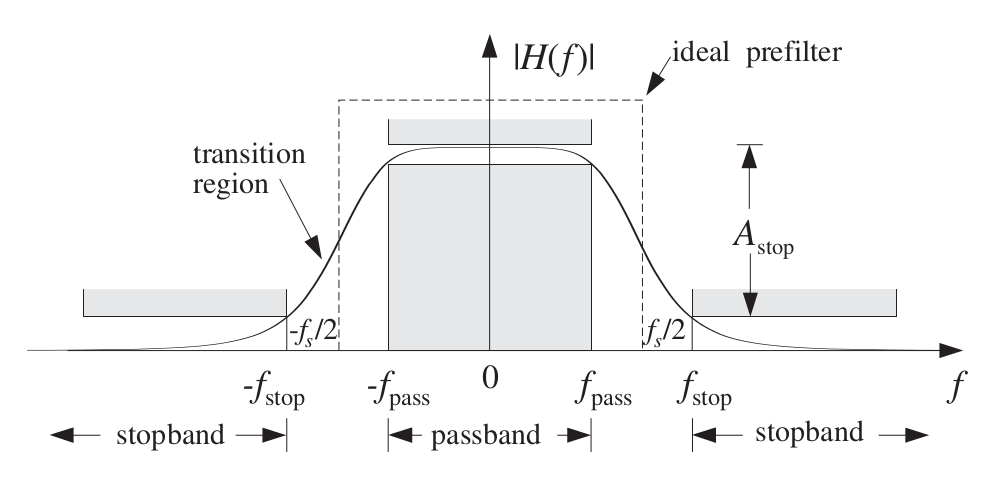
\includegraphics[width=9.5cm]{./picture/antialiasing_prefilter}

\end{multicols}

$f_0$: reference frequency (typ. DC)

\subsection{Reconstructors \buchSeite{42}}
\subsubsection{Ideal reconstructor \buchSeite{43}}
  \begin{tabular}{p{5cm}p{4cm}p{6cm}}
	  $H(f) = \left\lbrace \begin{matrix}
	    T & |f| \leq \frac{f_s}{2} \\
	    0 & else
	  \end{matrix}\right.$ & 
    $h(t) = \dfrac{\sin(\pi f_s t)}{\pi f_s t}$ &
    $y(t) = \sum\limits_{n=-\infty}^\infty y(nT)h(t-nT)$
  \end{tabular}
  

\subsubsection{Staircase reconstructor \buchSeite{45}}
  \begin{tabular}{p{8cm}p{8cm}}
    $h(t) = u(t) - u(t-T) = \left\lbrace \begin{matrix}
      1 & 0\leq t \leq T \\
      0 & else
    \end{matrix}\right.$ &
    $H(f) = \dfrac{1}{2\pi j f}(1-e^{-2\pi f T}) = T \cdot \dfrac{\sin(\pi f T}{\pi f T}\cdot e^{-\pi j f T}$
  \end{tabular}
  
  The spectral images at higher frequencies are not well suppressed, therefore an \textbf{anti-image postfilter} is needed.\\
  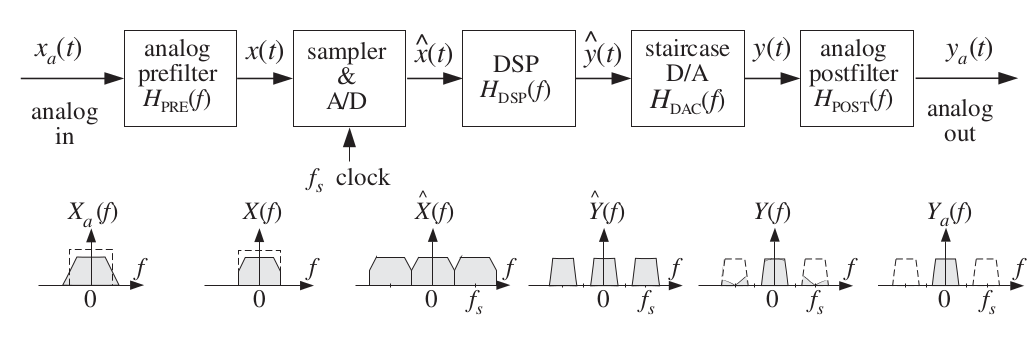
\includegraphics[width=16cm]{./picture/compOfDSPSystem}
  

  
  
